\section{Controller design} \label{sec:ctrl-design}
The main purpose of this chapter is firstly to discuss the reasoning behind using the LQR controller along with a presentation of the basic LQR and LQI theory. Then the derived LQI controller if shown and finally the LQI controller's effect on the system is analysed with respect to how the closed loop system poles move when LQI weights are changed. The controller to be derived is used in full state feedback and outputs a pitch reference to the system. Therefore the FLC controller is later removed from the model such that the input to the system is the pitch reference $ thRef $ instead of the rotor speed reference $ wRef $.

\subsection{Linear-Quadratic Regulator} \label{sec:ctrl_lqr}
The Linear-Quadratic Regulator (LQR) in its \textit{infinite horizon} form is the preferred controller type. LQR is chosen because satisfactory performance can be gained reasonably fast with some state and input weight tuning. Furthermore penalizing state deviations by the use of \textit{Bryson's Rule} can give an intuitive starting point for weights. Another common alternative, the \textit{pole placement method}, is disregarded as it can suffer from being less intuitive with regards to choosing the placement of poles. Furthermore an LQR controller guarantees 6 dB gain margin and 60 degree phase margin \cite{Doyle1978}. 

\smallskip
\noindent Consider the system:
\begin{equation}\label{eq:ctrl_sys}
	\begin{split}
		\dot x &= A x + B u \\
		y &= Cx
	\end{split}
\end{equation}
For such a system the LQR controller is optimal with respect to a relevant cost function such as:
\begin{equation}\label{eq:lqr_cost}
	J = \int_{0}^{\infty} \left(x^T Q x + u^T R u + 2x^T N u\right) dt
\end{equation}
where
\begin{center}
	\begin{tabular}{l r l }
		weight & $R$         & $ > 0$\hspace{1mm} (positive definite) and symmetric       \\
		weight & $Q$		 & $\ge 0$\hspace{1mm} (positive semi-definite) and symmetric
	\end{tabular}
\end{center}
\smallskip
The final cross-term which punishes combinations of inputs and states is usually omitted by setting $ N = 0 $. The entries of $ R $ and $ Q $ are considered tuning parameters. The solution to the LQR control problem is the optimal control feedback $ u = -Kx $ which minimizes the cost function. The LQR controller is thus inherently a regulator meaning that it drives the system states to 0. For a system linearised at an operating point (OP) $ \{x_o, u_o\} $ the state and input deviations from the OP replaces the actual states and inputs: $ \hat x = x-x_o $ and $ \hat u = u-u_o $. Given that the OP is located at the reference, the regulator property is obviously not unattractive. With $ N = 0 $ and states substituted with state deviations the final continuous-time cost function becomes:
\begin{equation}\label{eq:lqr_cost_final}
	J = \int_{0}^{\infty} \left(\hat x^T Q \hat x + \hat u^T R \hat u\right) dt
\end{equation}
The optimal feedback gain can be shown to be: 
\begin{equation}\label{eq:lqr_K}
	K = -R^{-1} B^T P
\end{equation}
with P being the solution to the algebraic Ricatti equation:
\begin{equation}\label{lqr:ricatti}
	A^T P + P A - P B R^{-1} B^T P + Q = 0
\end{equation}
It is noted that proving \cref{eq:lqr_K} is deemed outside the scope of this report. This leaves $ Q $ and $ R $ to be tuned in such a manner that a satisfactory performance is achieved. For initial guesses \textit{Bryson's Rule} can be utilized. It states that a diagonal entry in $ Q $ or $ R $ for a corresponding state $ x_i $ or input $ u_i $ should be set as such:
\begin{equation}\label{eq:bryson}
	\begin{split}
		Q_i = \dfrac{1}{Max(\hat x_i)^2} \\
		R_i = \dfrac{1}{Max(\hat u_i)^2}
	\end{split}
\end{equation}
where $ Max(\hat x) $ is the largest tolerated value of $ \hat x $. While optimal performance is rarely achieved without further tuning, Bryson's Rule gives a good starting point. In Matlab the \textit{lqr(A, B, Q, R, N)} function is used to get the controller gains $ K $.


\subsection{Linear-Quadratic Integrator} \label{sec:ctrl_lqi}
As described \cref{sec:comp_flc} the FLC controller is of the proportional-integrator (PI) type which ensures no generator speed steady state error due to integral action. The controller to be derived includes generator speed control and the regular LQR controller does not have integral action. Therefore the system is augmented with an integral state on the generator speed $ \dot x_i = \hat \omega $ leaving the extended state space system to be:
\begin{align} 
	\dot {\bar x} & = \begin{bmatrix} \dot{\hat x} \\ \dot x_i \end{bmatrix} = \begin{bmatrix} A &0 \\ C_{iy} & 0 \end{bmatrix} \bar x + \begin{bmatrix} B_u \\ 0 \end{bmatrix}  \hat u \\
	\bar y & = \begin{bmatrix} C & 0 \end{bmatrix} \bar x
\end{align}
where $ C_{iy} $ is defined such that the desired output is picked out for integration and $ \bar x $ is the deviation state vector extended with the integral state.

A linear quadratic integrator (LQI) controller is obtained when the integrator-augmented system matrices are used to solve the LQR problem. The dimension of $ Q $ increases for every extra integrator state and thus extra weights are defined for these. While Bryson's Rule is utilized for more intuitive definitions of weights on states and inputs, the integrator state weight is a far more awkward weight to choose. In this report it is set based on a tuning process as a multiple of the original state.


\subsection{The controller} \label{sec:ctrl_thecontroller}
In the preceding sections the LQR and LQI controllers were explained and we are therefore ready to make the LQI controller. Stability and controllability are checked and the system is both stable and controllable. The \textit{lqr()} Matlab function is used with the integrator-augmented system. Bryson's Rule is used to define $ Q $ and $ R $ by defining maximum limits to the states and controllable inputs. A less intuitive weight is put on the integrator state. After a controller tuning process in VTS the resulting gains are:
\begin{equation}\label{eq:lqi_K}
	K = \begin{bmatrix} -1.264 &  1.249 & -75.159 & -9.549 \end{bmatrix}
\end{equation}
when the $ Q $ and $ R $ matrices are defined as such:
\begin{equation}\label{eq:lqi_Q_and_R}
	\begin{split}
		Q = \begin{bmatrix}
			\dfrac{1}{max(p_y)^2}& 0 					& 0 															& 0 \cr
			0 					& \dfrac{1}{max(v_y)^2}	& 0 															& 0 \cr
			0 					& 0 					& \dfrac{1}{\left( max(\Omega) \cdot \frac{2 \pi}{60} \right)^2} & 0 \cr
			0 					& 0 					& 0 															& \dfrac{1}{(5 \cdot max(\Omega) \cdot \frac{2 \pi}{60})^2} \end{bmatrix} & = \begin{bmatrix}
			\dfrac{1}{5^2} 	&  	0 				&  0 										&  0 \cr
			0 				&  \dfrac{1}{1^2}	&  0 										&  0 \cr
			0 				&  0 				& \dfrac{1}{\left( 1 \cdot \frac{2 \pi}{60} \right)^2} 	&  0 \cr
			0 				&  0 				&  0 										&  \dfrac{1}{(5 \cdot \frac{2 \pi}{60})^2}
		\end{bmatrix} \\\\
		R = \begin{bmatrix} \dfrac{1}{\max(\theta_{ref})^2} \end{bmatrix} &= \begin{bmatrix} \dfrac{1}{5^2} \end{bmatrix}
	\end{split}
\end{equation}
From $ Q $ and $ R $ it is observable that:
\begin{itemize}
	\item the maximum allowed fore-aft position deviation is set to 5 m
	\item the maximum allowed fore-aft velocity deviation is set to 1 m/s
	\item the maximum allowed rotor speed deviation is set to 1 rpm
	\item the rotor speed integration weight is set 5 times lower than the rotor speed
	\item the maximum allowed pitch angle actuation deviation is set to 5 deg
\end{itemize}
The maximum tolerated rotor speed is multiplied with $ 2 \pi $/$ 60 $ to translate the weight from rpm to rad/s which is the state unit. There is furthermore no intuitive explanation behind the choice of the integrator weight other than that it has yielded satisfactory results in the controller tuning process. Only light tuning was necessary from the initial guesses of maximum tolerable state and input values to achieve good performance. This is regarded as a highlight of the usefulness of the LQR controller when a well fitting linear model is used. Also perhaps importantly when the necessary system understanding has not been achieved such that pole placement can be done based on reasonable design considerations. Some system understanding can perhaps be achieved by considering the positions of system poles and zeros and thus a drawback of LQR might be that some understanding is lost when omitting this process.
%\begin{equation}\label{eq:lqi_Q_and_R}
%	Q =   \begin{bmatrix}
%		0.04 &  0 &  0 &  0 \cr
%		0 &  1 &  0 &  0 \cr
%		0 &  0 & 91.1 &  0 \cr
%		0 &  0 &  0 &  3.65
%	\end{bmatrix}
%	 \;\; and \;\; 
%	R = \begin{bmatrix} 0.04 \end{bmatrix}
%\end{equation}



%s_W = 1; s_py = 5; s_vy = 1; s_Wi = s_W*5; s_th = 5;
%var_Omega	= (s_W * (2*pi)/60)^2;	% Permitted variance of Omega in [rad/s]
%var_py		= s_py^2;				% Permitted variance of py in [m]
%var_vy		= s_vy^2;				% Permitted variance of vy in [m/s]
%Qlqr = [1/var_py	0			0
%0			1/var_vy	0
%0			0			1/var_Omega];


%\begin{equation}\label{eq:lqi_Q_and_R}
%	Q =   \begin{bmatrix}
%		\dfrac{1}{5^2} 	&  	0 				&  0 										&  0 \cr
%		0 				&  \dfrac{1}{1^2}	&  0 										&  0 \cr
%		0 				&  0 				& \dfrac{1}{\left( 1 \cdot \frac{2 \pi}{60} \right)^2} 	&  0 \cr
%		0 				&  0 				&  0 										&  \dfrac{1}{(5 \cdot \dfrac{2 \pi}{60})^2}
%	\end{bmatrix}
%	\;\; and \;\; 
%	R = \begin{bmatrix} \dfrac{1}{5^2} \end{bmatrix}
%\end{equation}

\subsection{LQI controller analysis}
This section is dedicated to analysing how the LQI controller moves the system poles and changes the system behaviour when some weights of $ Q $ and $ R $ are changed. The poles of the open-loop uncontrolled system is plotted together with the closed-loop LQI controlled system. Each plot contains a change in one weight (e.g. via $ max(\Omega) $) with three variations of that weight to see how the poles move. The weights which are not changed are left at the tuned values presented in \cref{sec:ctrl_thecontroller}. 

\begin{figure}[ht]
	\centering
	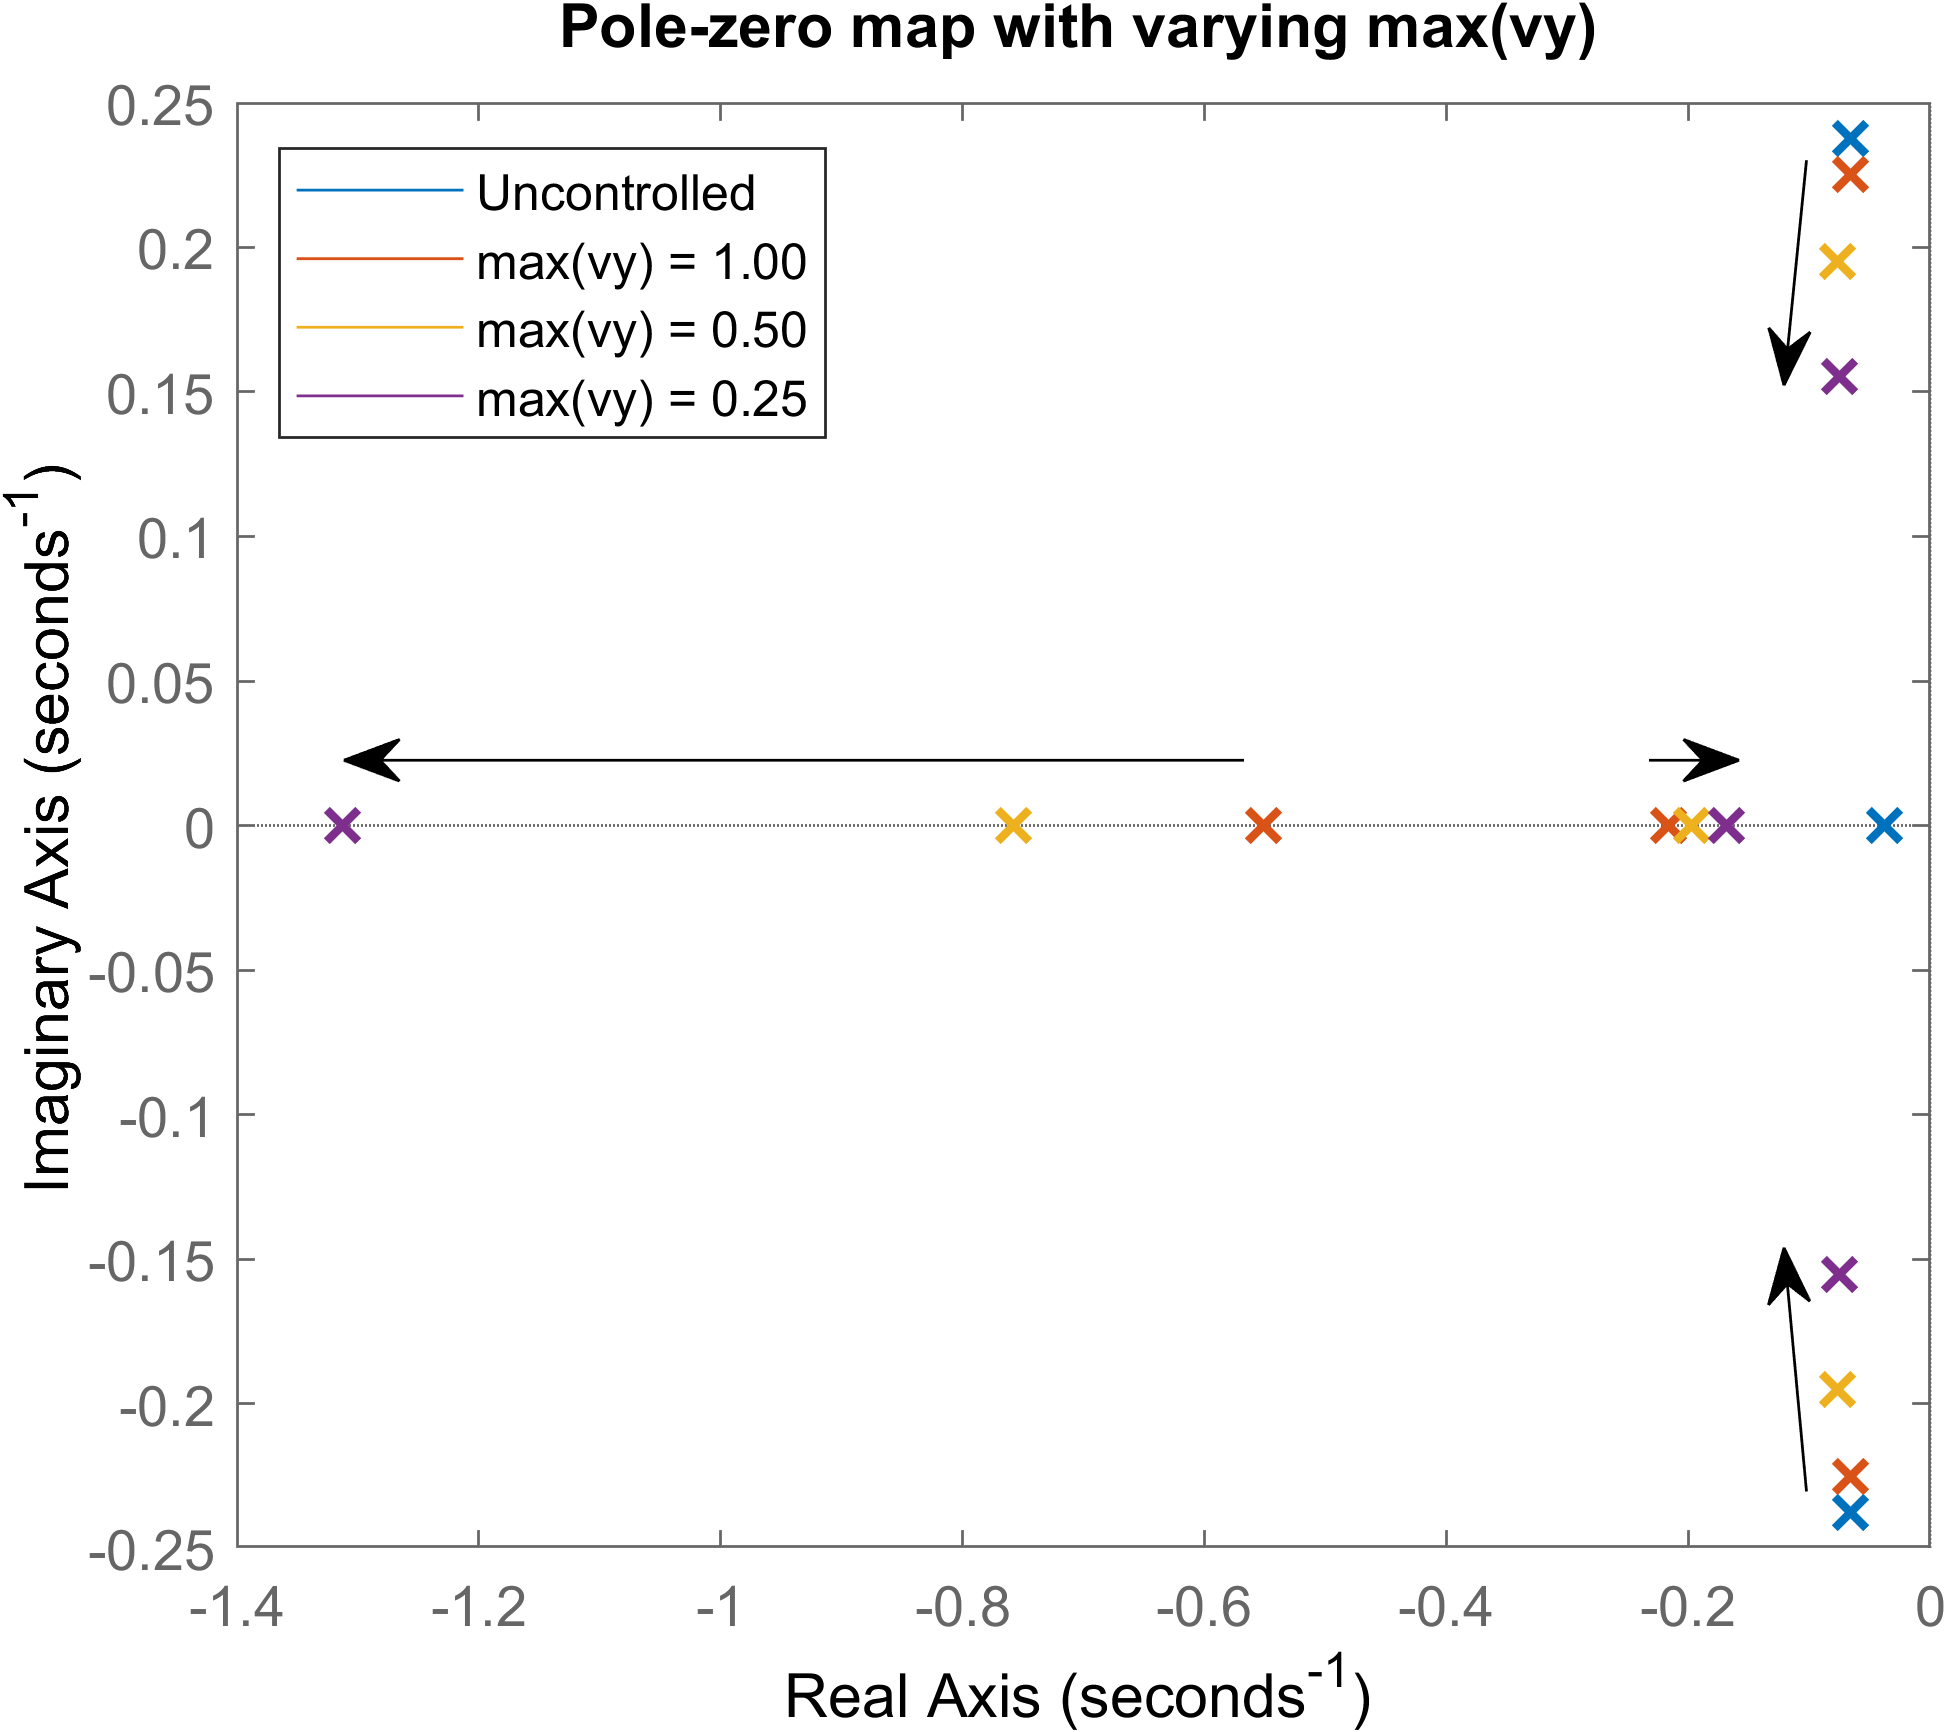
\includegraphics[width=.55\textwidth]{Graphics/LQI pole zero/02_pzmap_vy}
	\caption{Pole-zero diagram with varying LQI weight on the state $ v_y $. Arrows indicate the pole movement direction tendency.}
	\label{fig:pzmap_vy}
\end{figure}
\begin{figure}[ht]
	\centering
	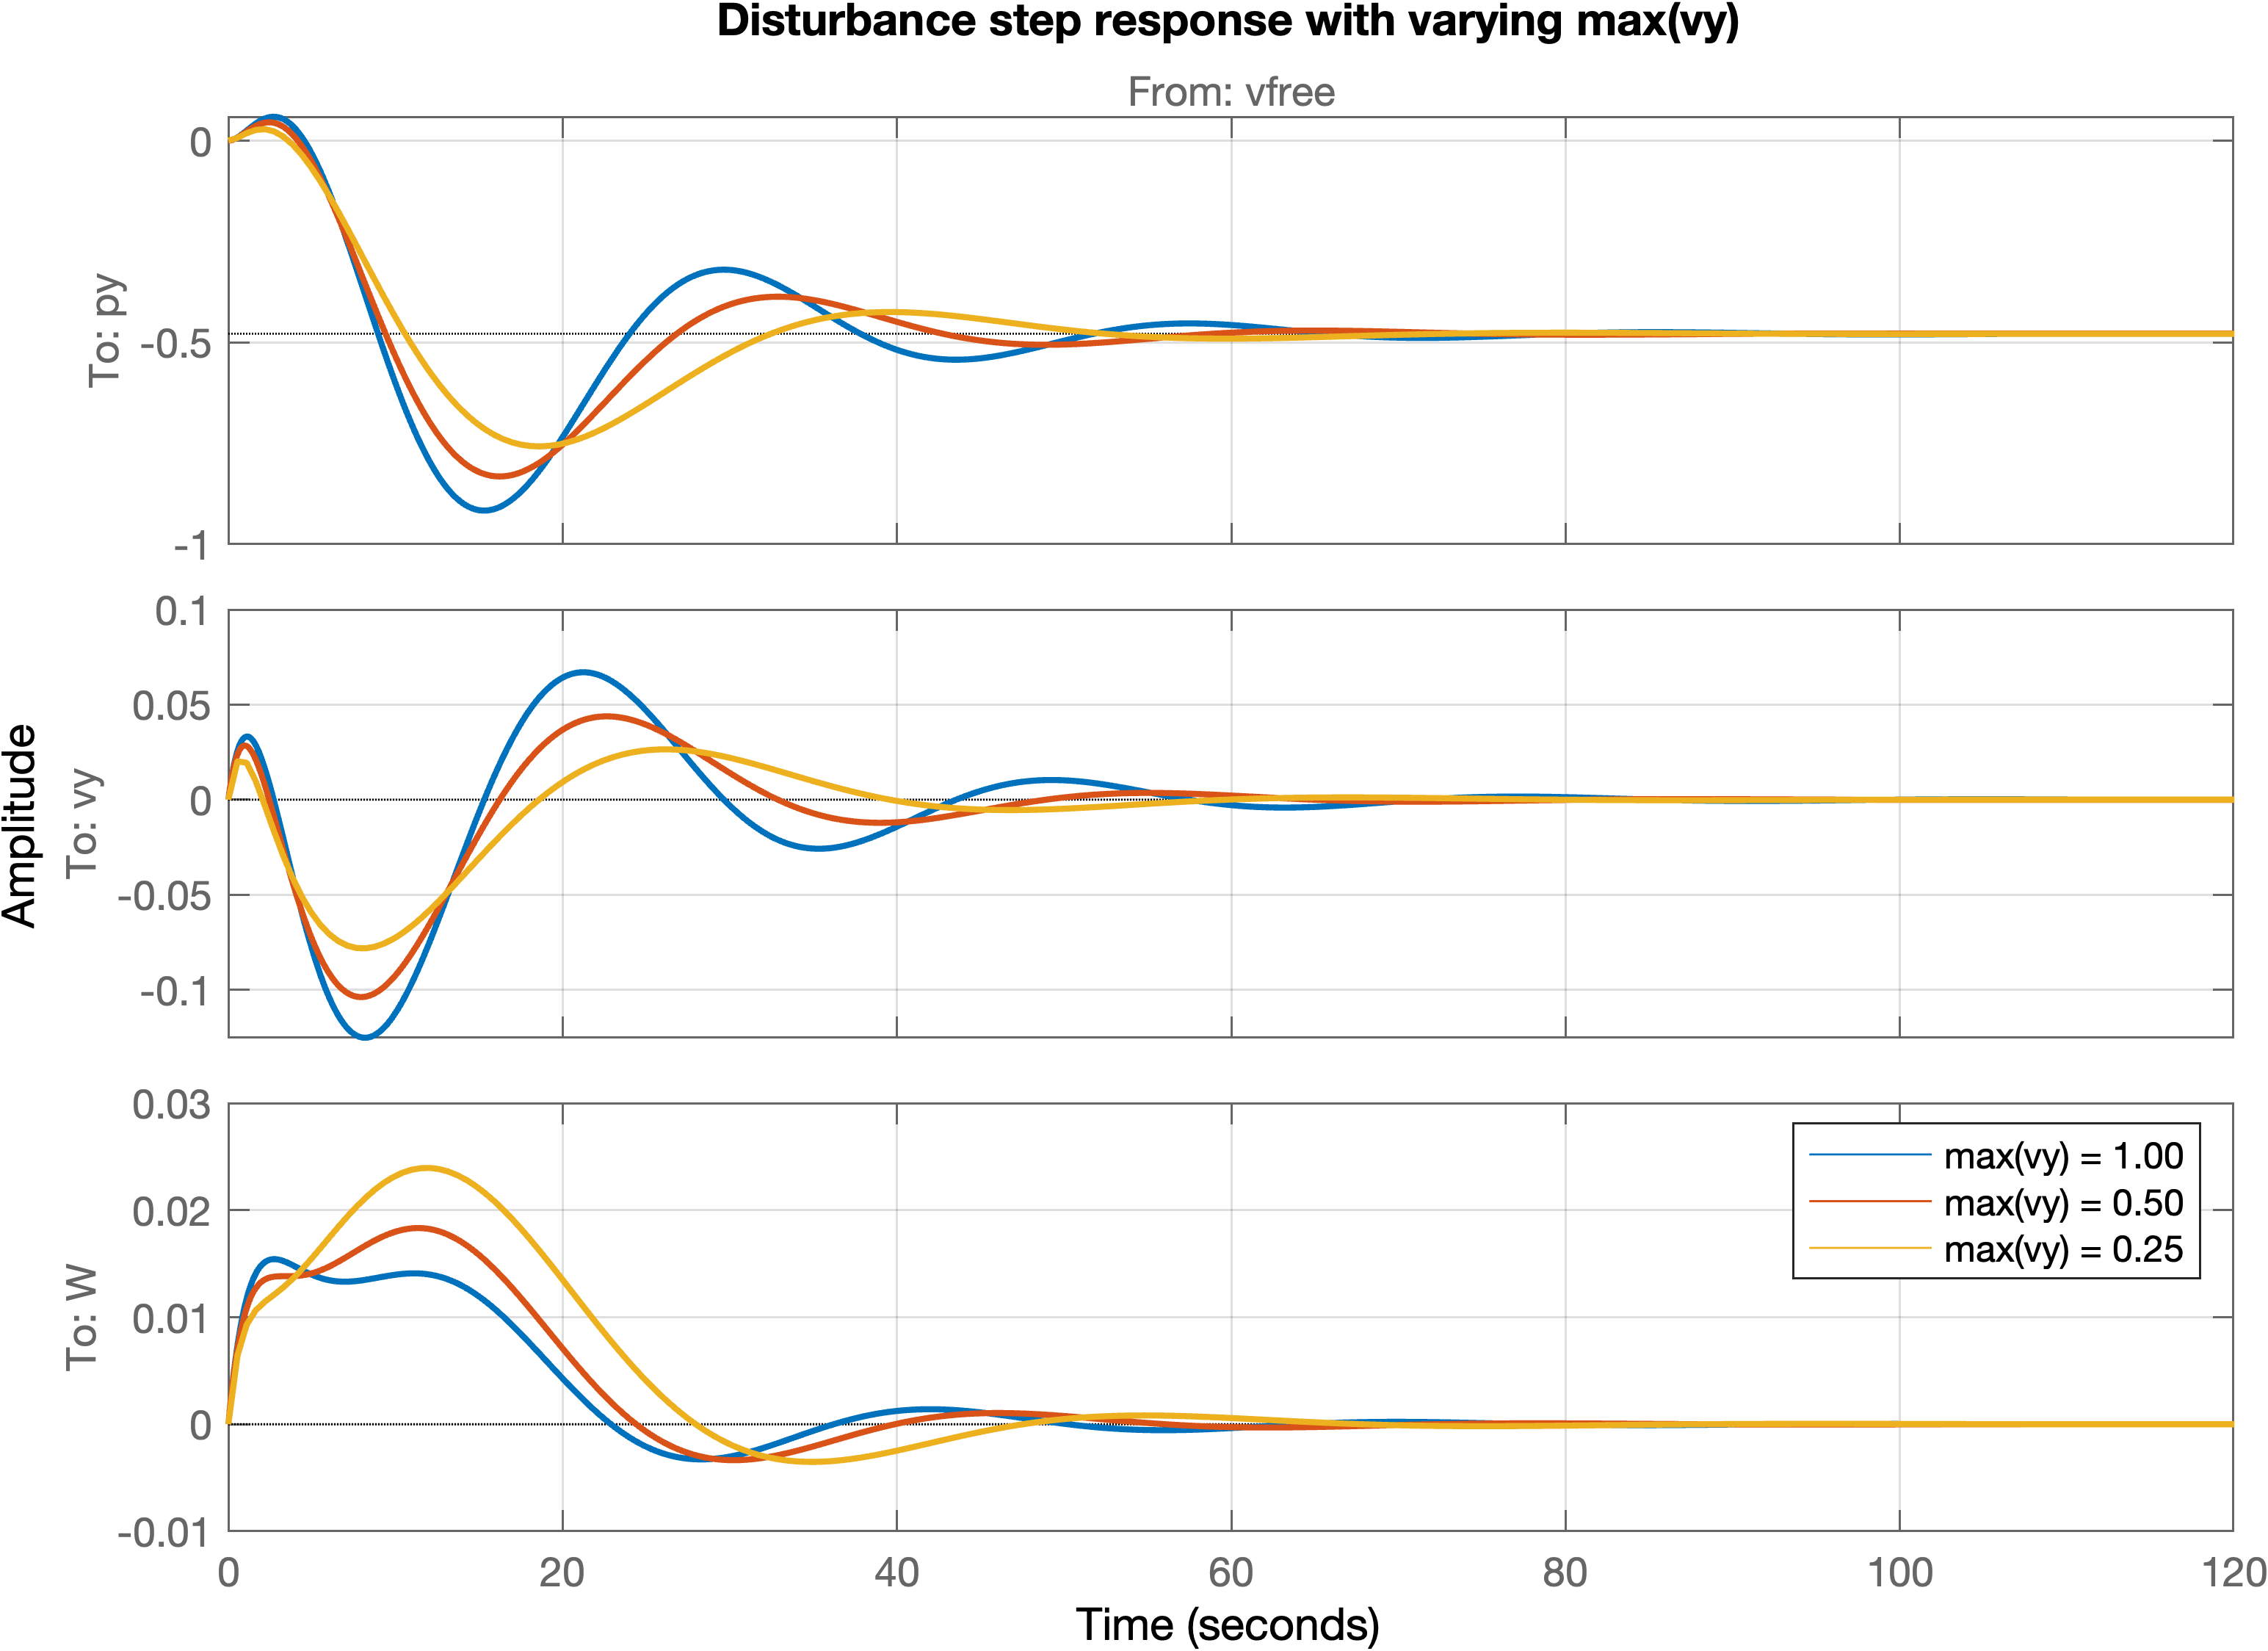
\includegraphics[width=0.7\textwidth]{Graphics/LQI pole zero/102_step_vy.png}
	\caption{Step response from a step on the free wind disturbance. The weight on $ v_y $ is varied. The y-axis shows the deviation from the OP. The rotor speed reference is at the OP and therefore the third subplot shows the rotor speed tracking error. An increased weight on the fore-aft velocity results in reduced fore-aft motion oscillations but greater rotor speed tracking error.}
	\label{fig:step_vy}
\end{figure}
In \cref{fig:pzmap_vy} the LQI $ Q $ weight on $ v_y $ is varied via $ 1/max(v_y)^2 $. The blue markers indicate the poles of the uncontrolled system which only has three poles due to the missing integrator state. The frequency of the pole pair closest to the imaginary axis fit well with the structure eigenfrequency around 0.035 Hz. The high ratio between the imaginary and real part indicate a very low dampening of especially the uncontrolled system (blue markers). As expected when putting a greater weight on the tower velocity the dampening is increased. It moves from 0.28 for $ max(vy) = 1 $ to 0.435 for $ max(vy) = 0.25 $. This happens because of the reduction of mainly the imaginary component of the dominating pole pair. The increased dampening is expected to lead to reduced oscillations of the turbine structure. This is also apparent when observing a step response as in \cref{fig:step_vy}. Here a reduction of the oscillations of $ p_y $ and $ v_y $ is observed but at the cost of a greater rotor tracking error. Furthermore, in the pole-zero diagram, the \textit{fastest} (most negative) pole on the real axis becomes even faster while the slowest becomes slower. The implications of how this affects the system response is harder to deduce. It is especially difficult to reason why the pole movement translates into the observed rotor speed response.

Furthermore one might wonder why the LQI controller does not simply make the dominating floating pole pair even faster with an even higher dampening. Here one should consider that a weight on the actuator effort is still in place (in the form of $ max(\theta_{ref}) = 5 $) which limits the possibility of extensively reducing the fore-aft motion.

\begin{figure*}[ht]
	\centering
	
	\subfloat[Pole-zero map]
	{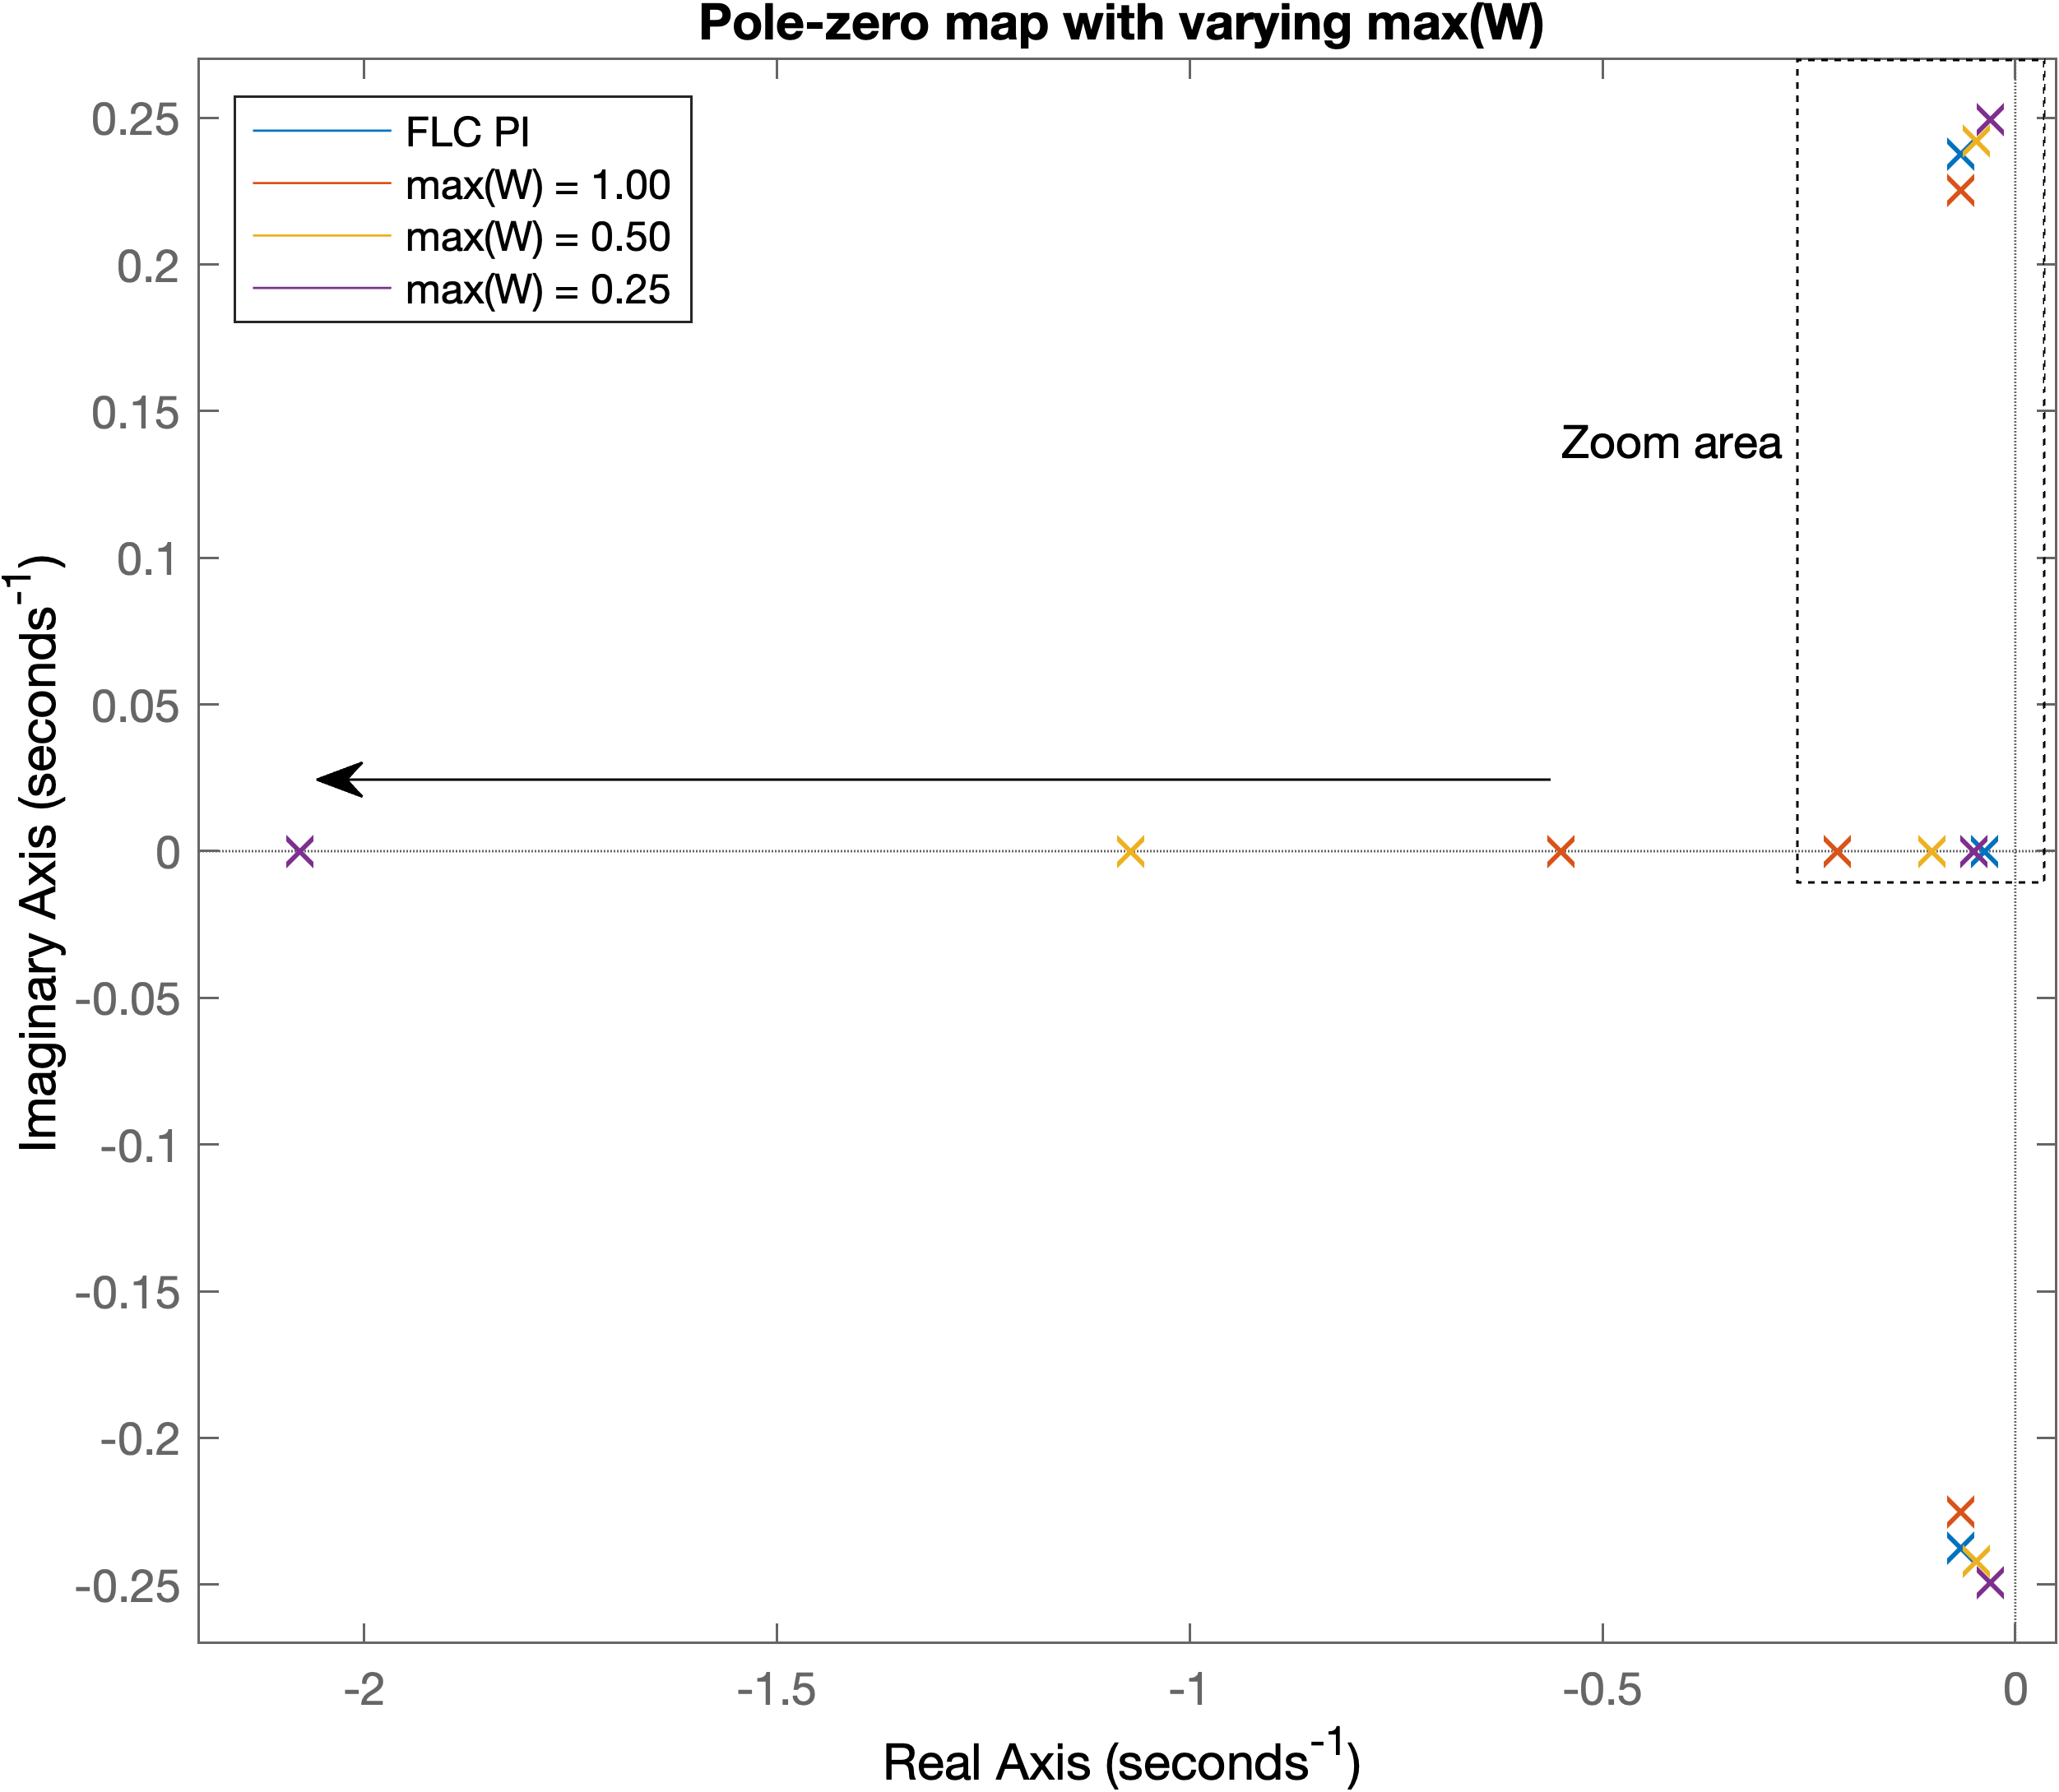
\includegraphics[width=.48\textwidth]{Graphics/LQI pole zero/03_pzmap_W}%
		\label{fig:pzmap_W}}
	\hfil
	\subfloat[Pole-zero map zoomed]
	{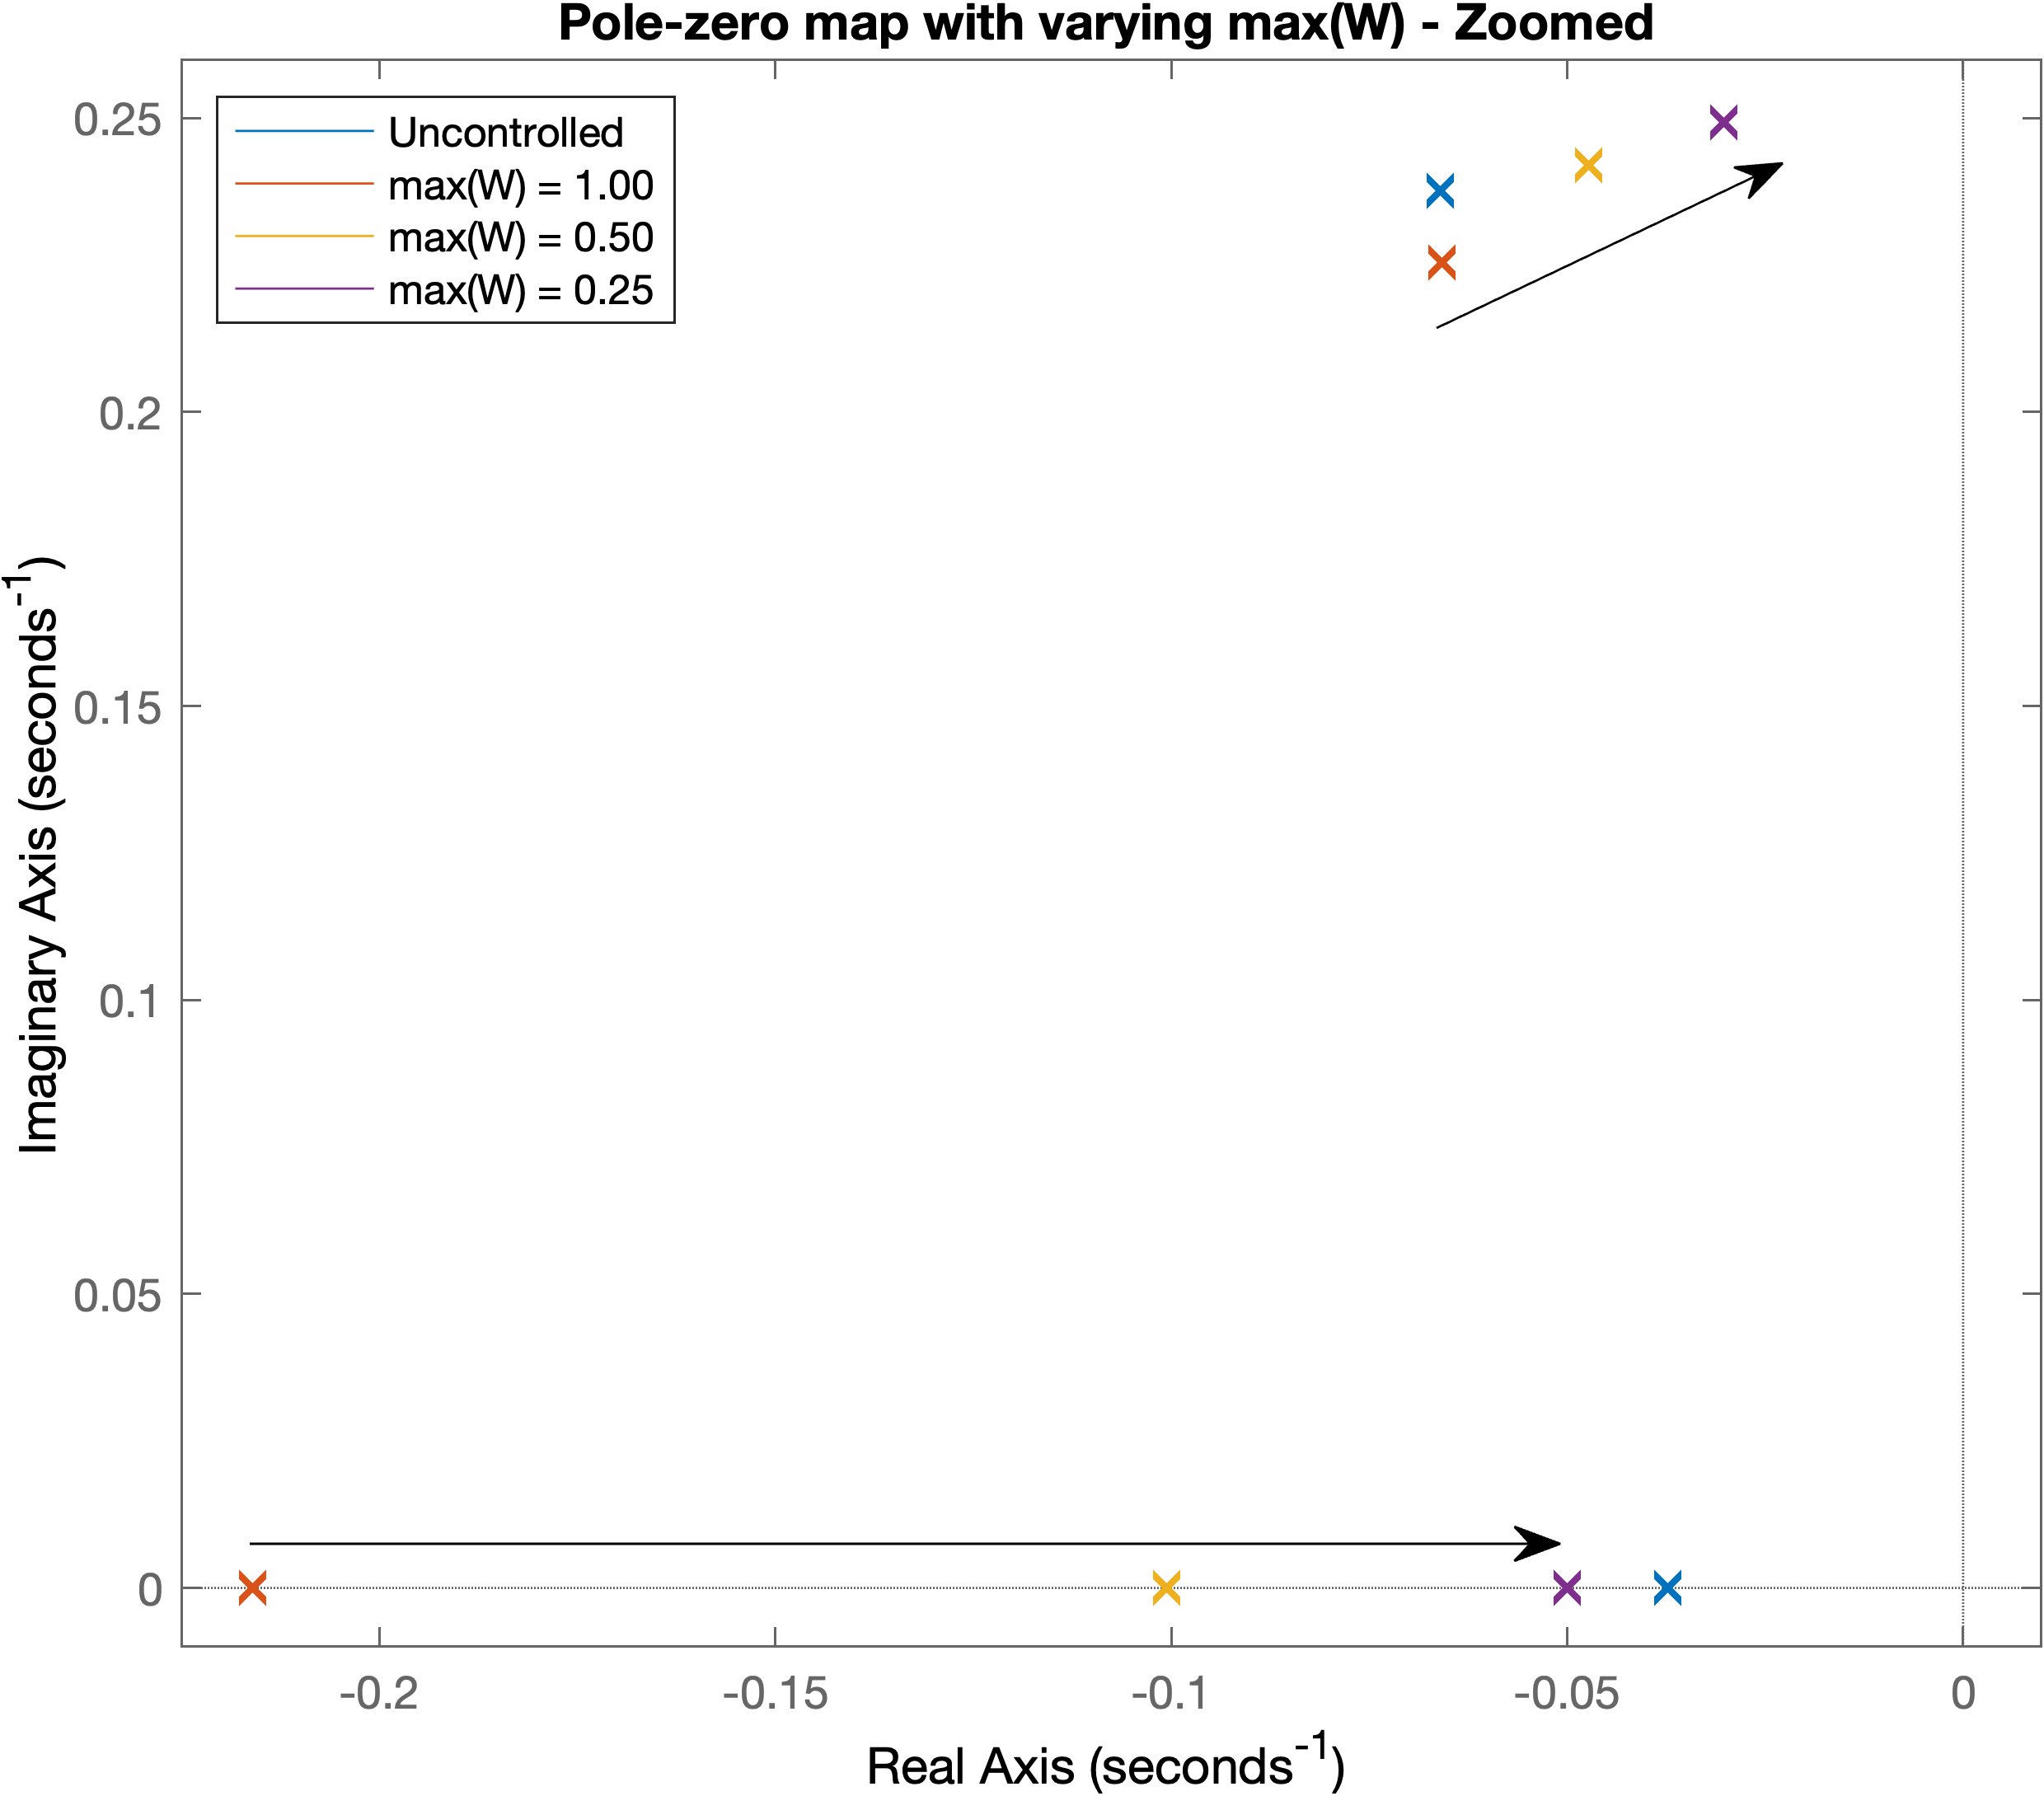
\includegraphics[width=.48\textwidth]{Graphics/LQI pole zero/13_pzmapzoom_W}%
		\label{fig:pzmap_W_zoom}}
	
	\caption{Pole-zero diagram with varying LQI weight of the state $ \Omega $; \textbf{(a)} Pole-zero plot; \textbf{(b)} Pole-zero plot zoomed at the indicated area.}
	\label{fig:pzmap_W_both}
\end{figure*}
In \cref{fig:pzmap_W_both} two plots are seen where the one in \cref{fig:pzmap_W_zoom} is zoomed in at the area indicated in the top right corner of \cref{fig:pzmap_W}. Here a greater weight is put on $ \Omega $ and in contrast to the $ v_y $ case the dominating pole pair of the floating structure moves in the opposite direction. This leads to lower dampening and stability of the floating movement due to the poles being closer to the imaginary axis. As expected when observing the step response in \cref{fig:step_W} the fore-aft oscillations are greater and last longer. Surprisingly the two poles located on the real axis move in the same direction as in \cref{fig:pzmap_vy} with the fastest pole becoming much faster and the slow pole becoming much slower. The effect as seen on the step response is that the rotor speed error is reduced. Giving a reasonable explanation for the movement of the poles on the real axis and how it yields better rotor speed tracking is difficult. With regards to the floating pole pair it is perhaps intuitive that if a much greater emphasis is put on limiting the rotor speed error it comes at the cost of less desirable fore-aft motion.

\begin{figure}[ht]
	\centering
	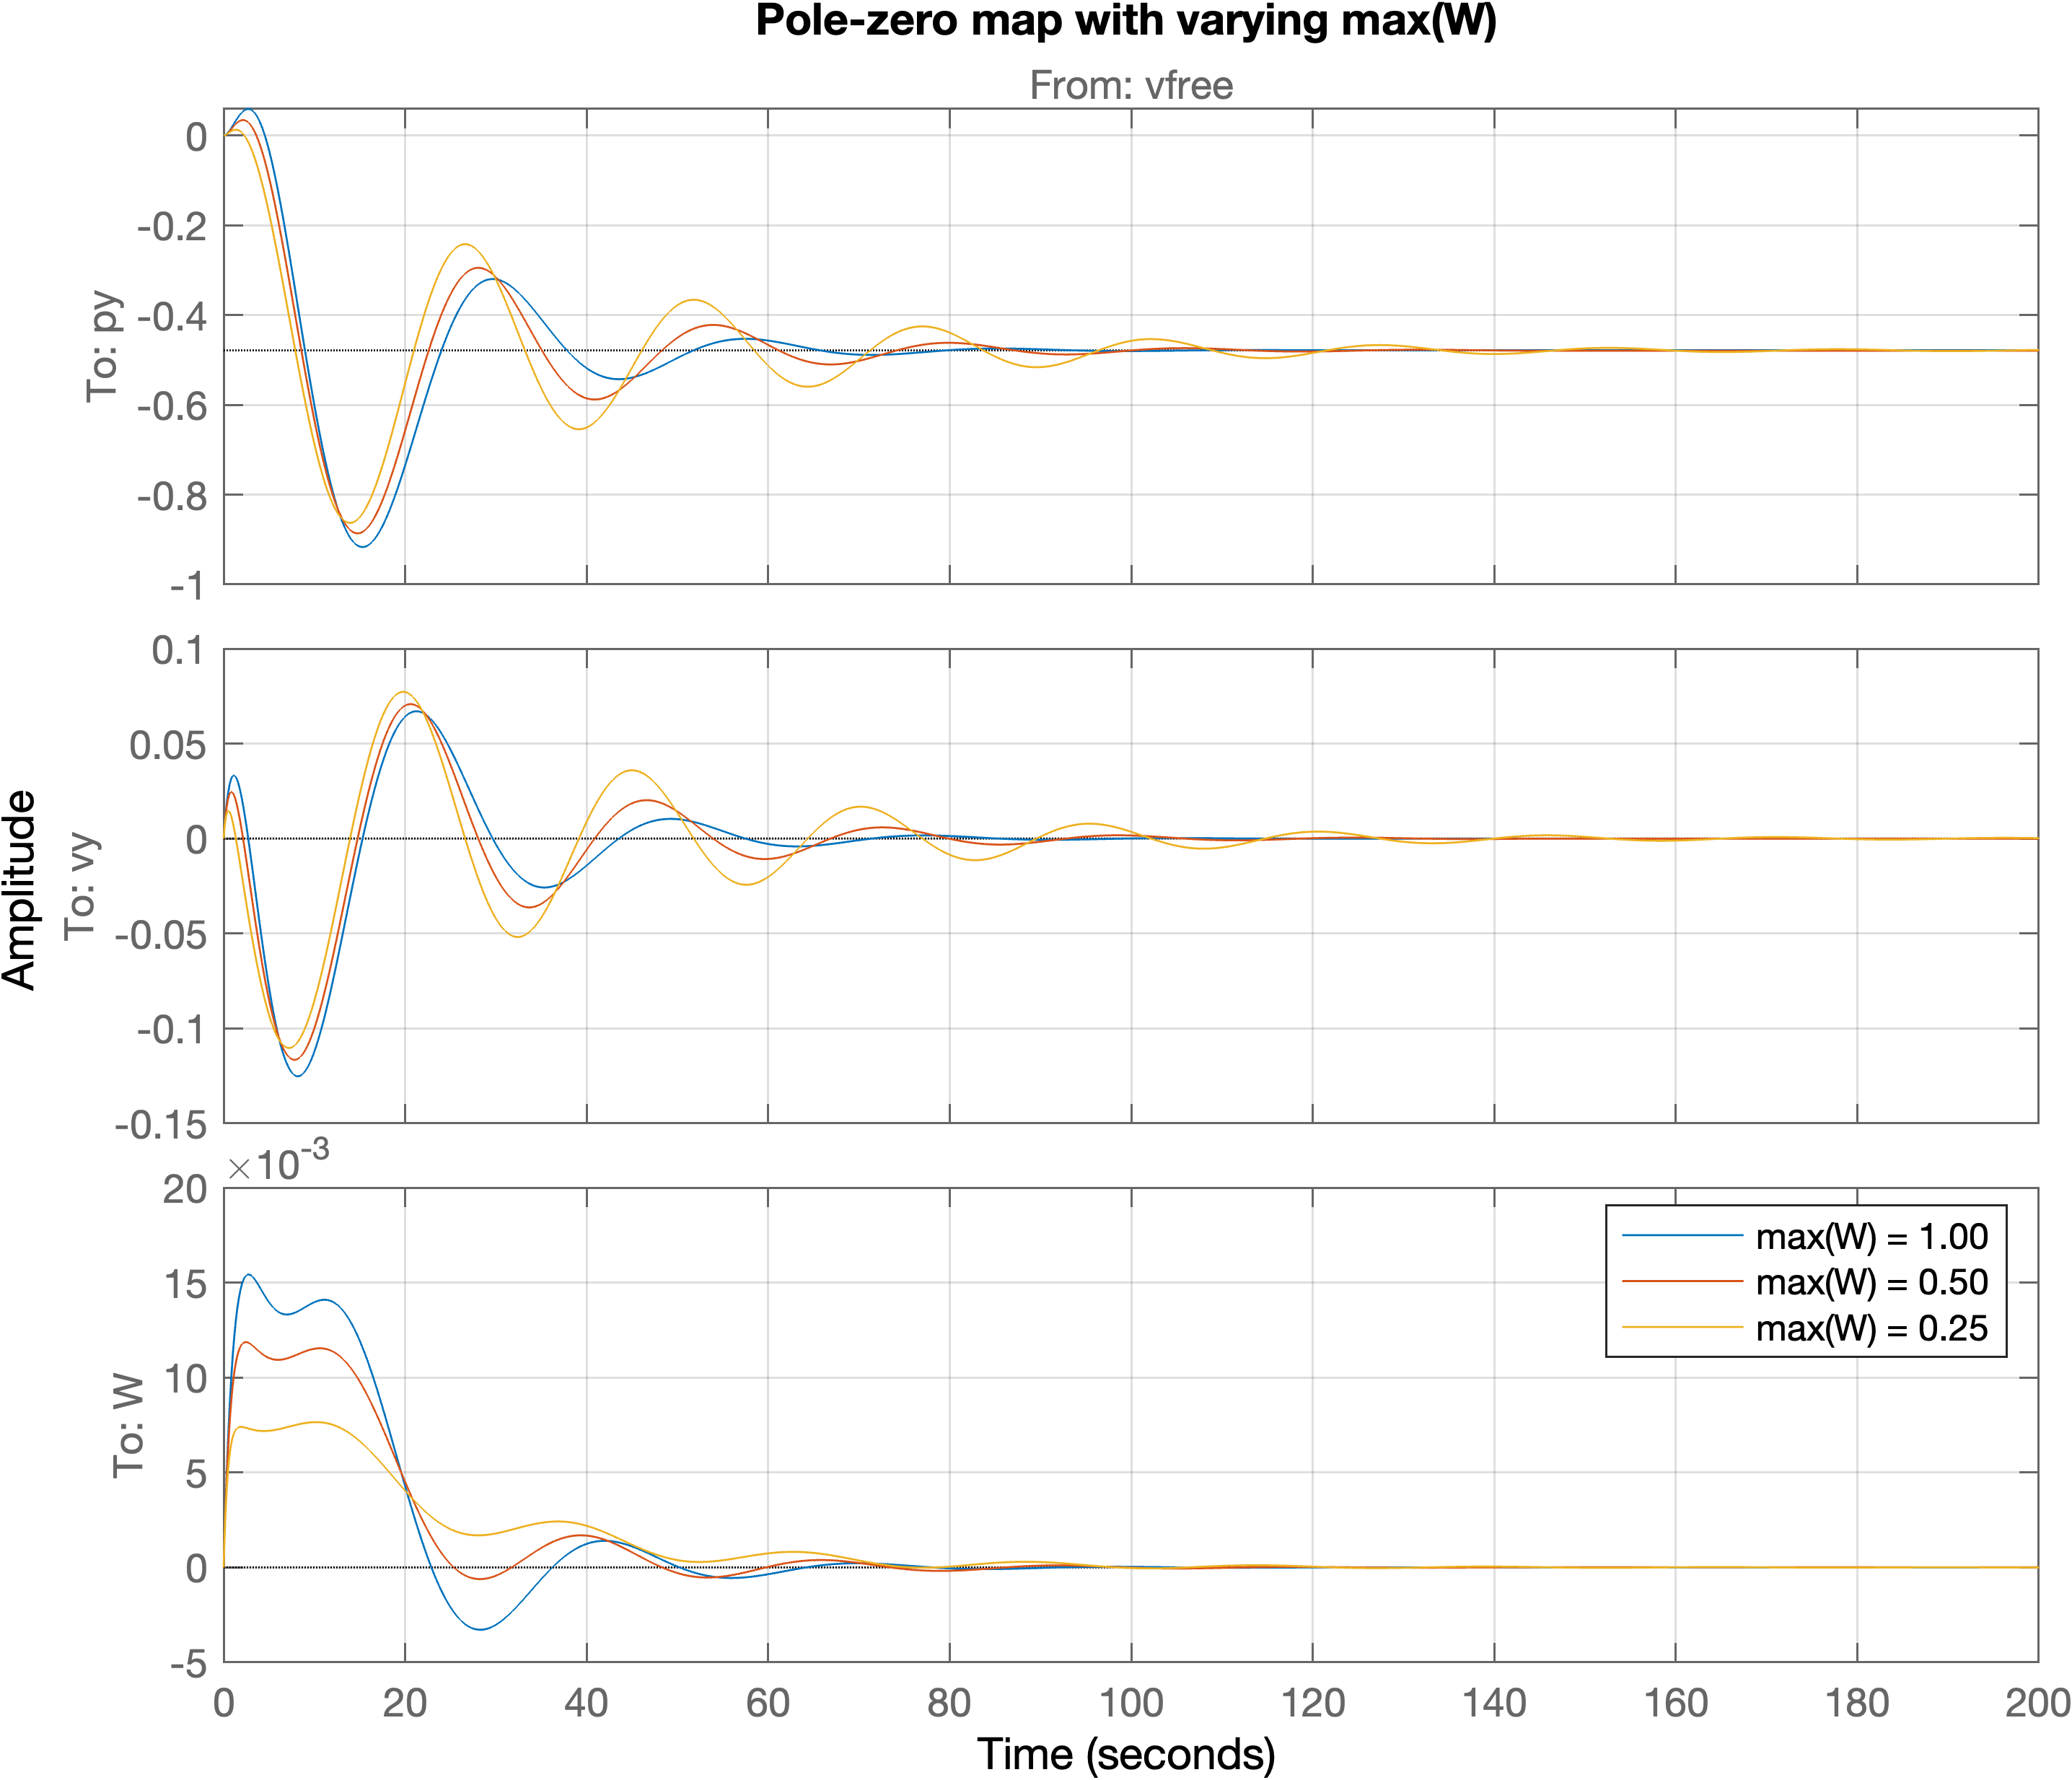
\includegraphics[width=0.7\textwidth]{Graphics/LQI pole zero/103_step_W.png}
	\caption{Step response from a step on the free wind disturbance. The weight on $ \Omega $ is varied. The y-axis shows the deviation from the OP. The rotor speed reference is at the OP and therefore the third subplot shows the rotor speed tracking error. An increased weight on the rotor speed tracking error yields slightly greater fore-aft motion oscillations but lower rotor speed tracking overshoot.}
	\label{fig:step_W}
\end{figure}

In \cref{fig:pzmap_theta} the maximum accepted value of the rotor pitch angle actuation is varied from 1 deg to 5 deg with 5 deg being the original tuned parameter. With a low accepted value of 1 deg the two poles which were located at the real axis have instead become a slower pole pair as observed by the red poles at $ -0.1 \pm0.8 $. As the "constraint" is relieved from 1 to 5 deg the pole pair becomes faster with a lower dampening and ultimately turns into two faster real poles. The dominating pole pair's imaginary part is furthermore lowered as the weight is decreased. The general tendency is that the system becomes both faster and more dampened. As expected allowing for a greater actuator effort leads to a better and faster system altogether which is also readily visible in the step response in \cref{fig:step_theta}. Both the magnitude of oscillations and settle time is reduces for both the tower movement and rotor speed error.
\begin{figure}[ht]
	\centering
	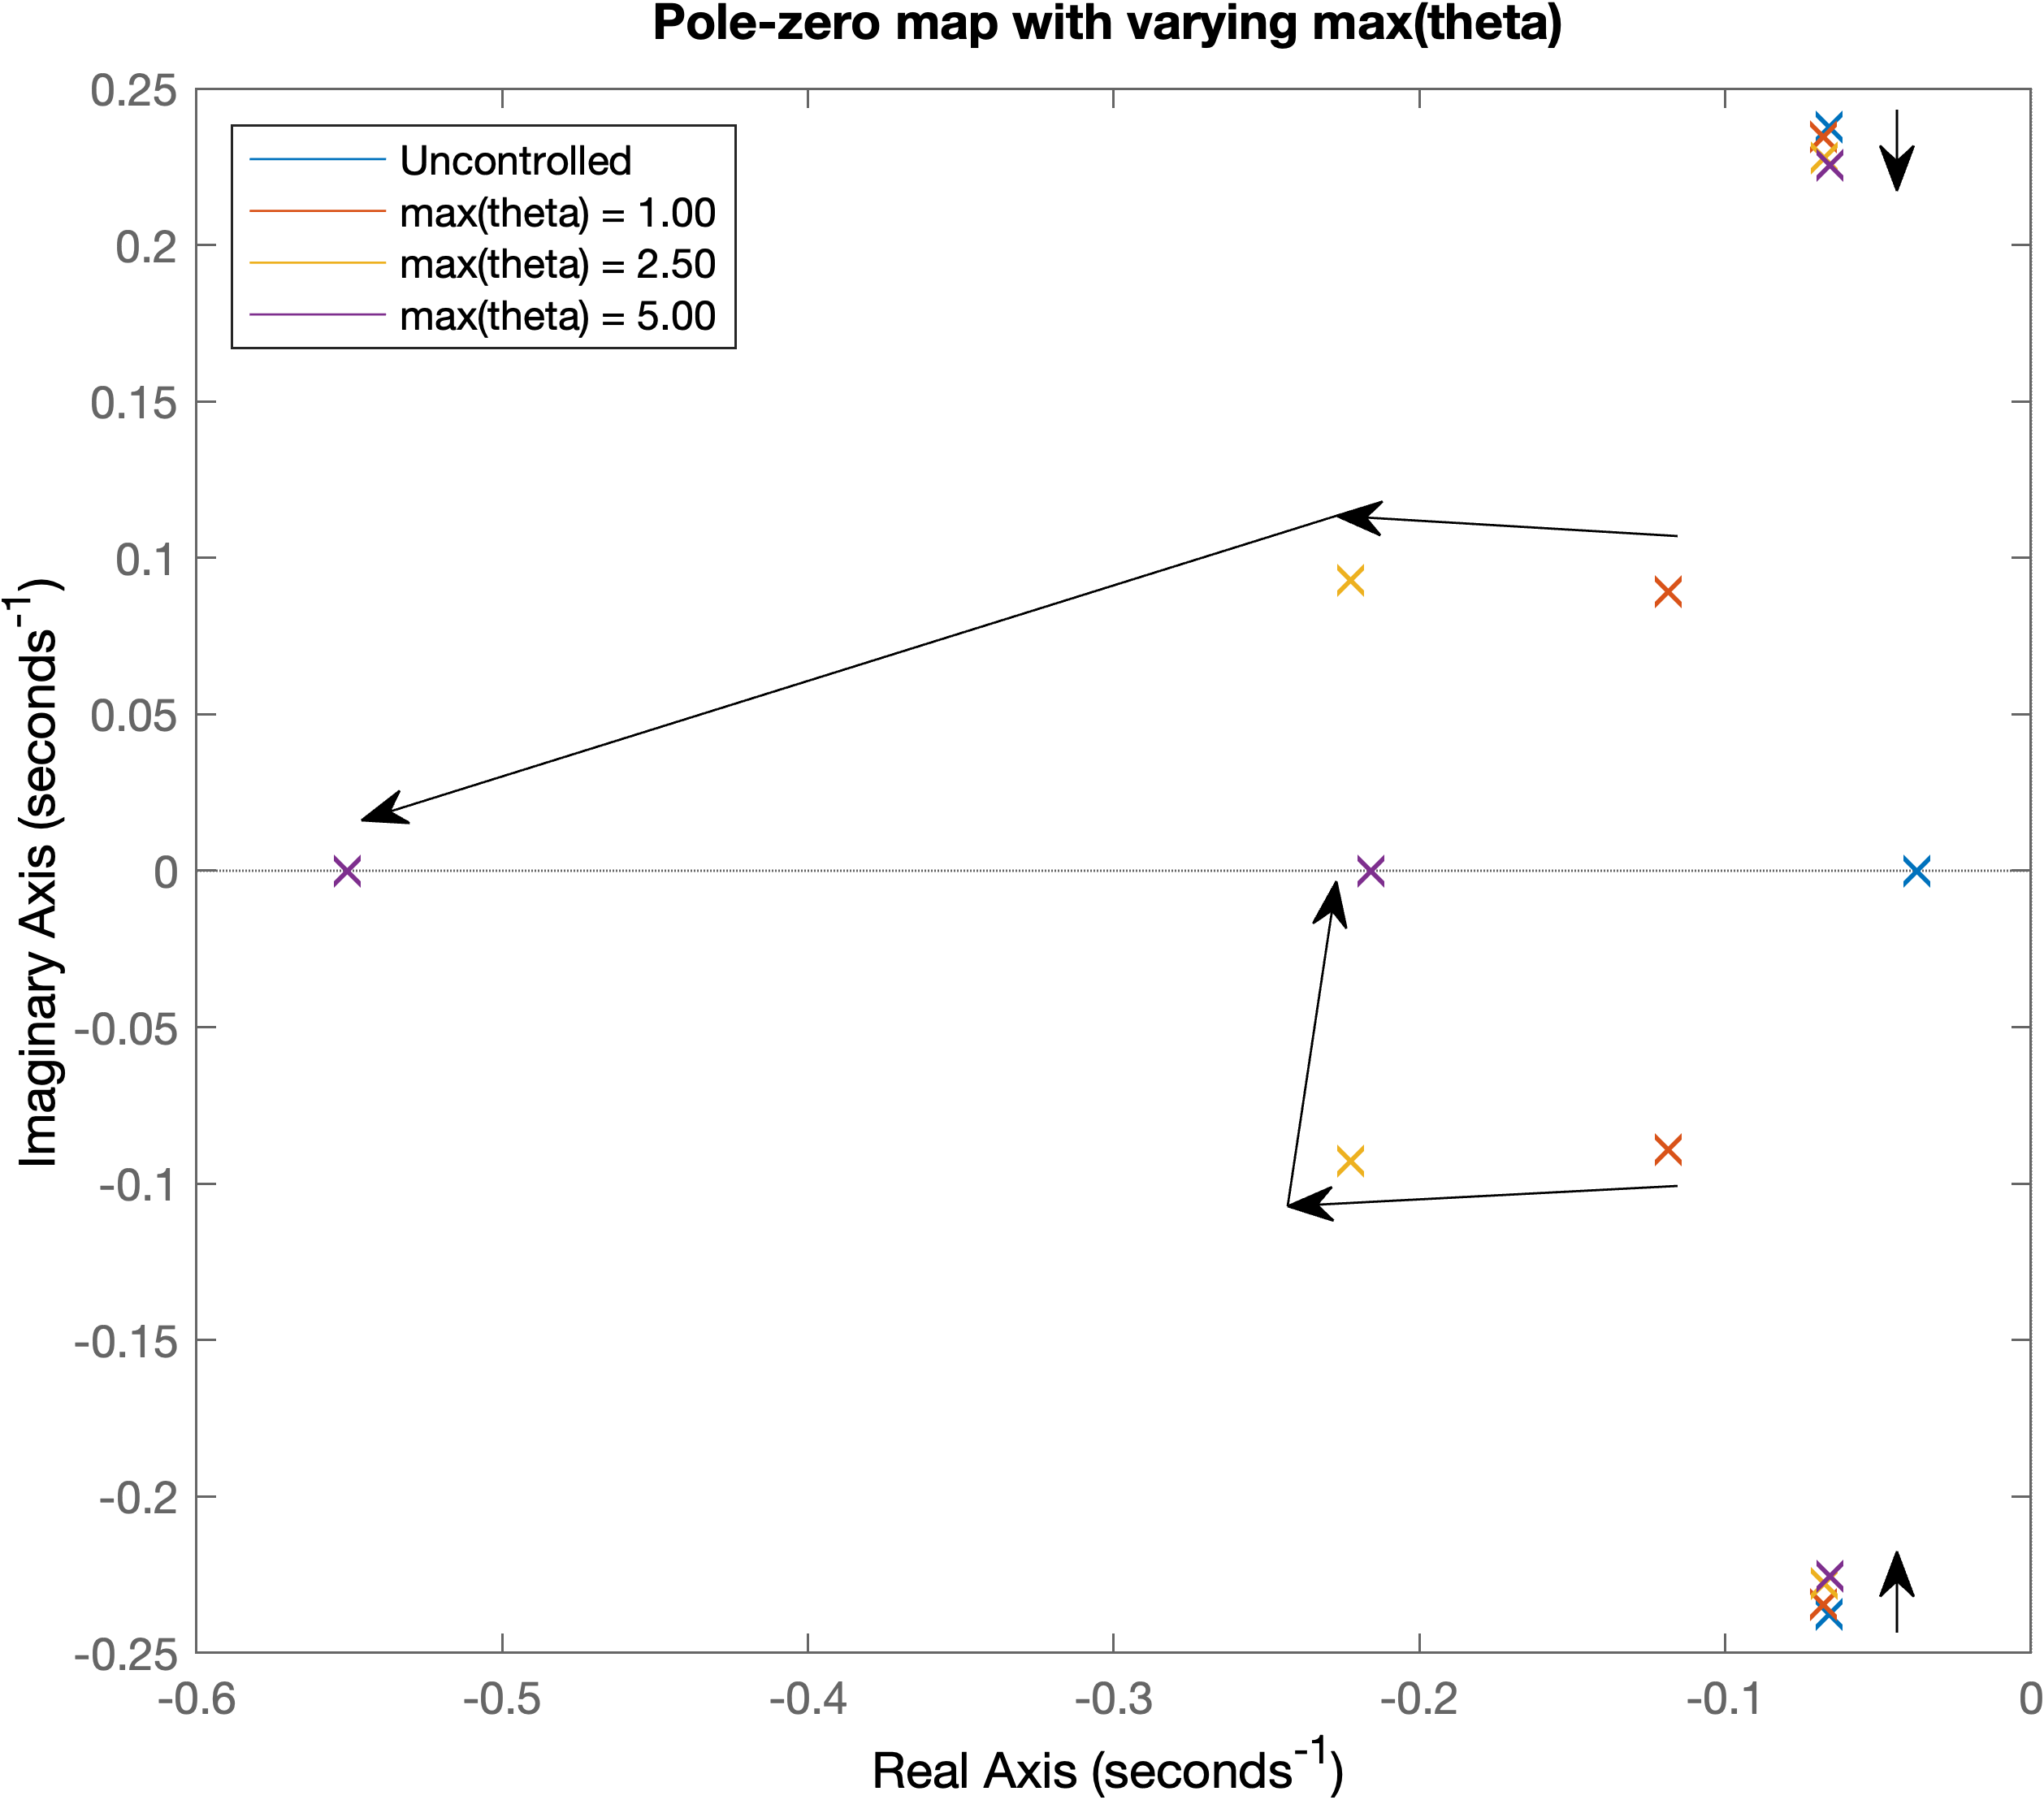
\includegraphics[width=0.55\textwidth]{Graphics/LQI pole zero/05_pzmap_theta.png}
	\caption{Pole-zero diagram with varying LQI weight on the actuator input $ \theta $.}
	\label{fig:pzmap_theta}
\end{figure}

\begin{figure}[ht]
	\centering
	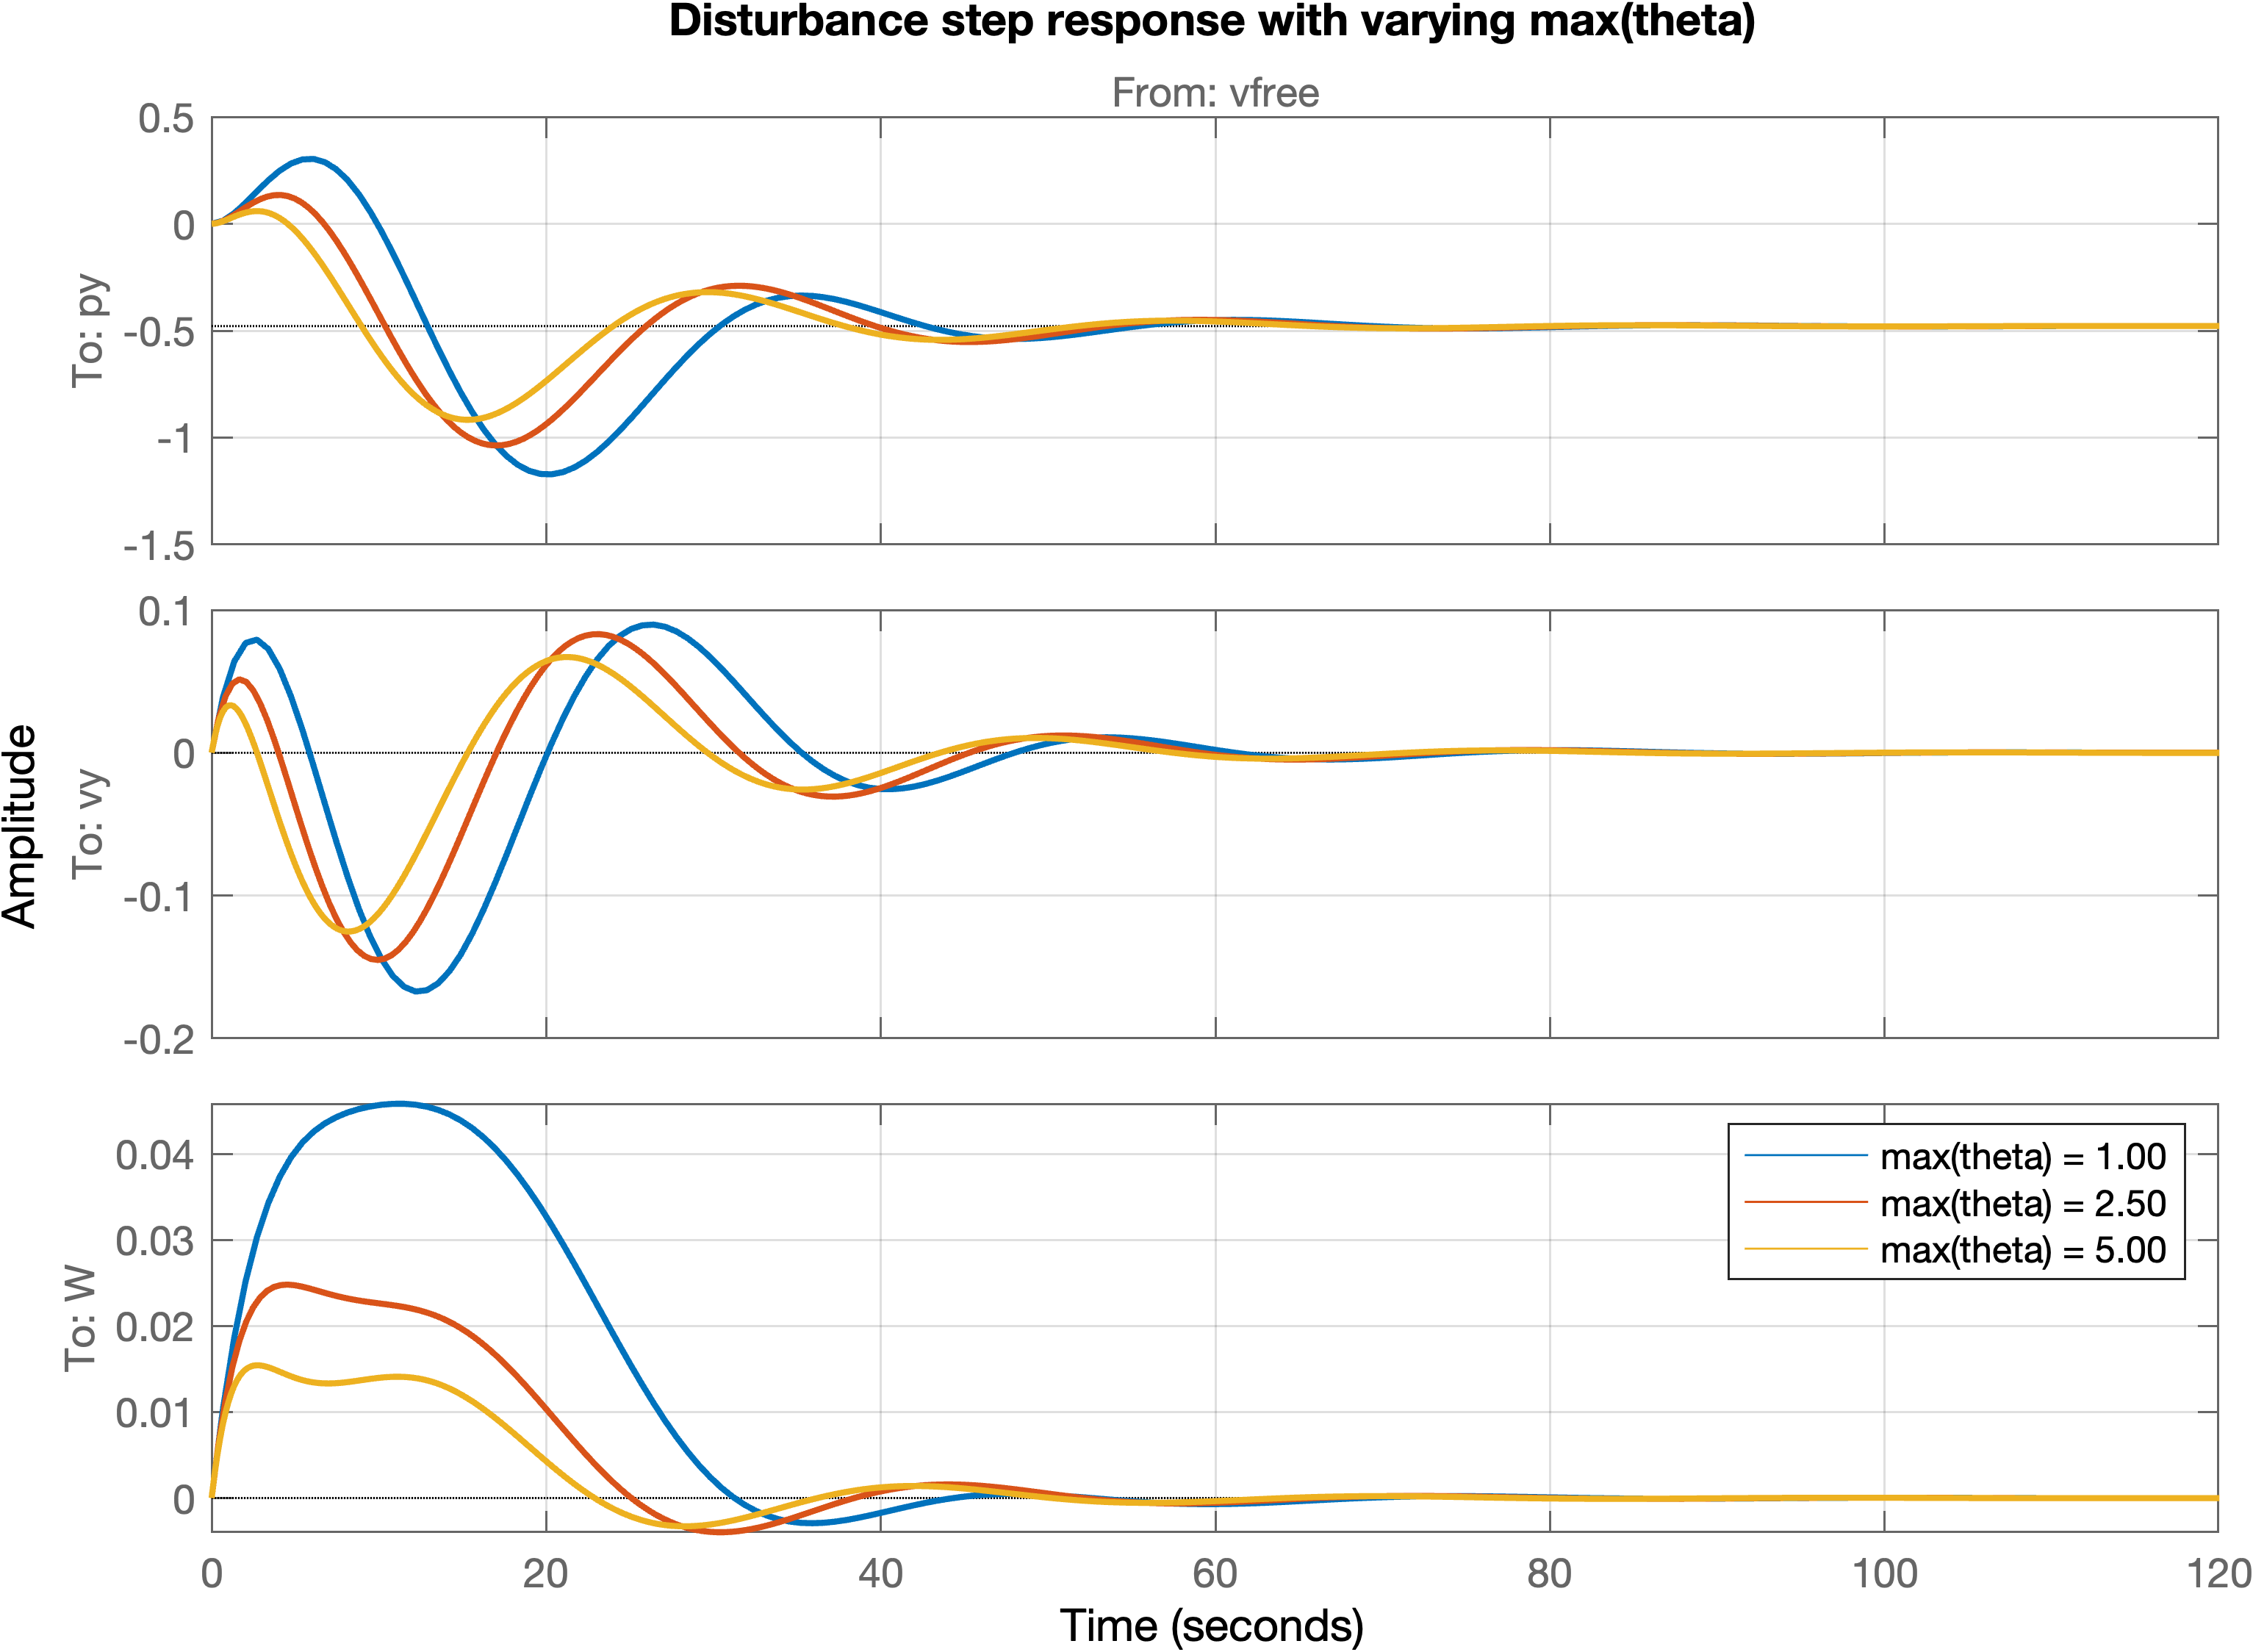
\includegraphics[width=0.7\textwidth]{Graphics/LQI pole zero/105_step_theta.png}
	\caption{Step response from a step on the free wind disturbance. The weight on $ \theta_{ref} $ is varied. The y-axis shows the deviation from the OP. The rotor speed reference is at the OP and therefore the third subplot shows the rotor speed tracking error. Lowered weights on the actuator effort results in both smaller fore-aft oscillations with lower settling time and smaller rotor speed tracking overshoot with slightly lower settling time.}
	\label{fig:step_theta}
\end{figure}


%\begin{figure*}[ht]
%	\centering
%	
%	\subfloat[sub-float1]
%	{\includegraphics[width=.49\textwidth]{Graphics/LQI pole zero/}%
%		\label{fig:1}}
%	\hfil
%	\subfloat[sub-float2]
%	{\includegraphics[width=.50\textwidth]{Graphics/LQI pole zero/}%
%		\label{fig:2}}
%	
%	\caption{Total text; \textbf{(a)} a-text; \textbf{(b)} b-text.}
%	\label{fig:3}
%\end{figure*}